%- block legend
Tanaka ganhou de presente de aniversário um relógio analógico, mas percebeu que ele não funcionava corretamente. Depois de observá-lo por um tempo, descobriu que sua função não era mostrar as horas, e sim ser um quebra-cabeça matemático. Tanaka adorou o presente, pois ama quebra-cabeças.
O desafio funciona da seguinte forma: o ponteiro das horas (desconsidere os demais ponteiros) começa apontando para as $12$h, em um mostrador cíclico numerado de $1$ a $12$. Um painel do relógio exibe uma hora $H$ e, em seguida, dois números $X$ e $Y$.
O quebra-cabeça consiste em duas perguntas independentes, ambas partindo do ponteiro na posição $12$: é possível, movendo-o exatamente $X$ vezes (cada movimento podendo ser em qualquer sentido, horário ou anti-horário), fazê-lo parar sobre a hora $H$? E, separadamente, é possível fazer o mesmo movendo-o exatamente $Y$ vezes?
\begin{center}
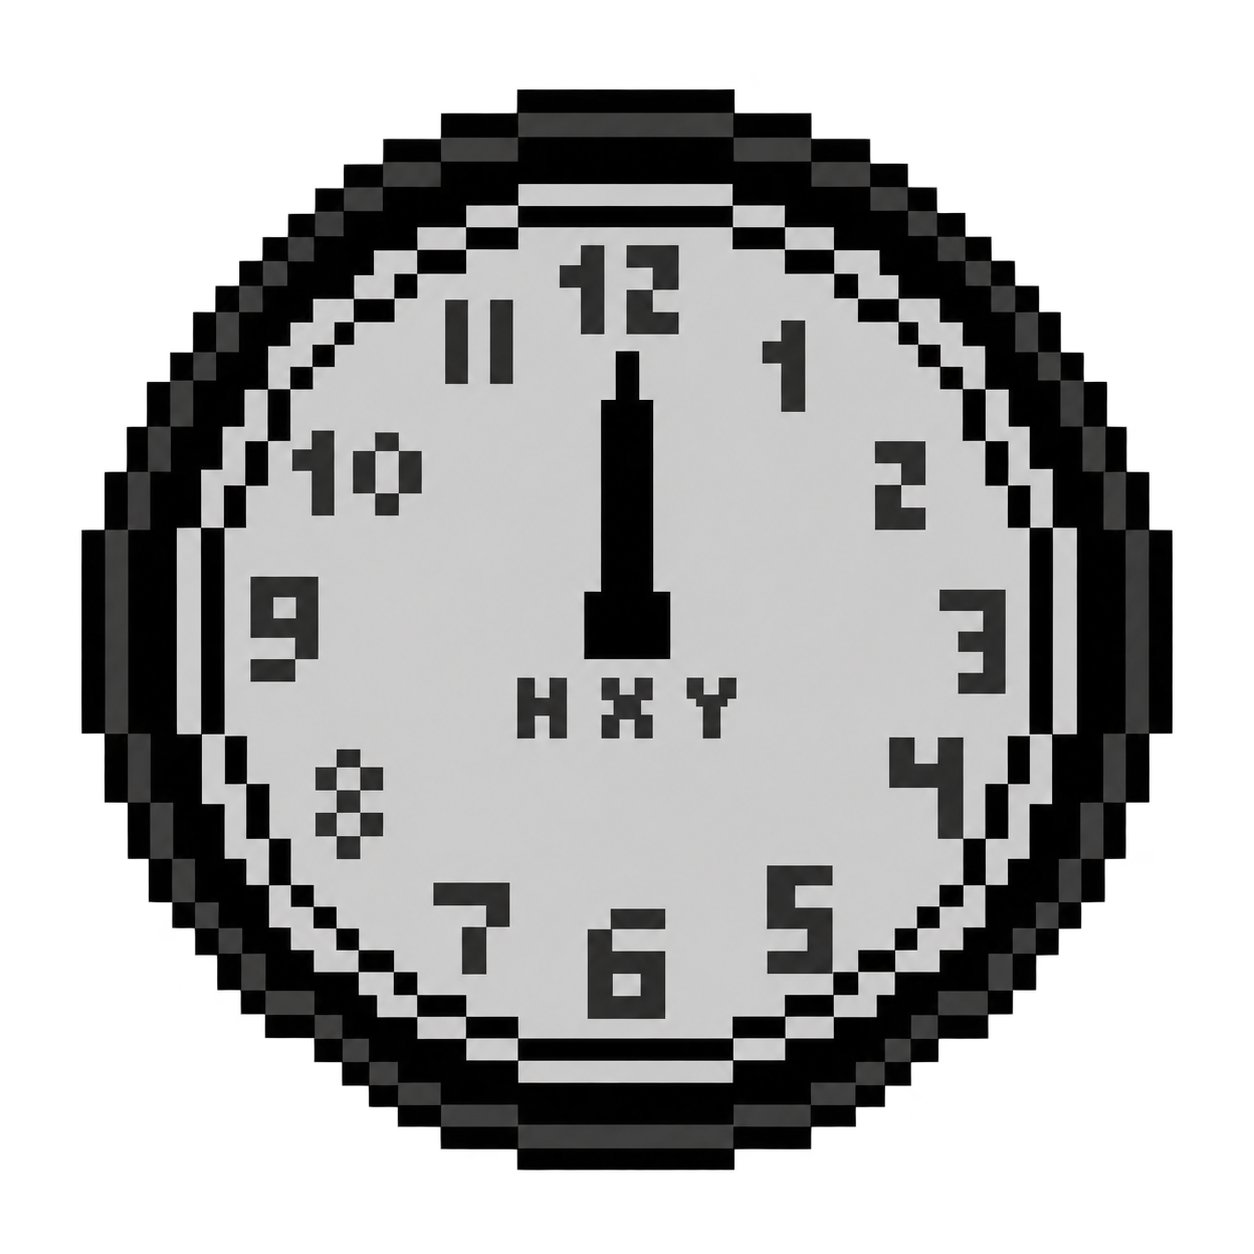
\includegraphics[scale=0.15]{clock.png}
\end{center}

%- endblock

%- block input
A entrada consiste em três inteiros $H$, $X$ e $Y$ ($1 \leq H \leq 12$, $1 \leq X, Y \leq 10^{18}$): a hora que se deseja alcançar e as quantidades de movimentos independentes a serem realizados com o ponteiro, respectivamente.
%- endblock

%- block output
Imprima "SIM"  caso seja possível levar o ponteiro, inicialmente na posição $12$, até a hora $H$ realizando $X$ movimentos e depois $Y$ movimentos; caso contrário, imprima "NAO".
%- endblock

%- block explanation_0
Neste exemplo podemos mover o ponteiro 6 vezes seguidas em qualquer sentido de modo que ele fique exatamente nas 6h.
%- endblock

%- block explanation_1
Neste exemplo para 4 movimentos é impossível chegar nas 7h pois a menor distância entre 7 e 12 no relógio é 5.
%- endblock

%- block editorial
Primeiramente observamos que para $X$ movimentos a partir da hora 12h só vamos conseguir terminar em um horário com a mesma paridade de $X$.
Por exemplo para $X = 1$ podemos mover para 11h ou 1h, ambas horas ímpar, para $X = 2$ podemos mover das 11h para 10h ou 12h das 1h para 12h ou 2h, ambas pares.
Verficando se a paridade permite chegar na hora $H$ verificamos em sequência se o valor de movimentos é maior ou igual a menor distância das 12h para $H$.
Complexidade: $O(1)$
%- endblock